\section{Vectors}
\noindent
A vector is a quantity with both direction and magnitude. One can think of it as a directed line segment. In multivariable calculus, we mostly will work with vectors in $\mathbb{R}^2$ and $\mathbb{R}^3$, but vectors can exist in other dimensions.\\

\noindent
Numerical (scalar) quantities have vector analogues, many of which show up in physics. Speed becomes velocity, distance becomes displacement, and mass becomes weight.\\

\noindent
Say we have a 2D vector, $\vec{v}=\langle v_x, v_y \rangle$.

\begin{figure}[h]
	\centering
	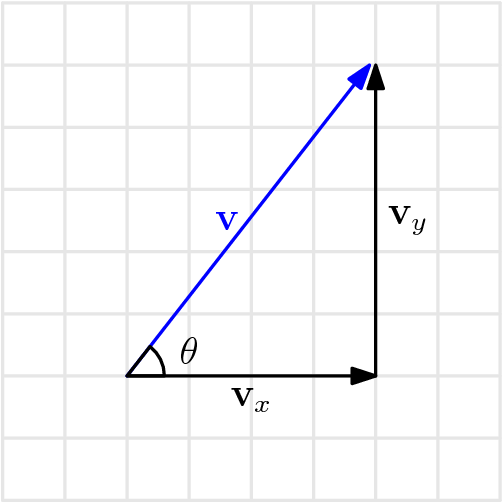
\includegraphics[scale=0.5]{Images/backgroundReview/VectorAddition}
\end{figure}

\noindent
Its length, also called magnitude or norm, is notated $\norm{\vec{v}}=\sqrt{v_x^2+v_y^2}$. This pattern of the norm being equal to the square-root of the sum of the squares of the vector's components continues into higher dimensions.\\

\noindent
The angle a 2D vector forms with the horizontal axis is $\theta = \tan^{-1}{\left(\frac{v_y}{v_x}\right)}$. There is not a useful version of this formula in higher dimensions.\\
Using $\theta$ and $\norm{\vec{v}}$, we can see that $v_x=\norm{\vec{v}}\cos{\theta}$ and $v_y=\norm{\vec{v}}\sin{\theta}$.\\

\noindent
Vectors can be added and subtracted from each other in a way that the result is another vector. We do this numerically by adding the corresponding components of each vector.\\
For example, if $\vec{a}=\langle 1,3 \rangle$ and $\vec{b}=\langle 4,7 \rangle$, then $\vec{a}+\vec{b}=\langle 1+4, 3+7 \rangle = \langle 5,10 \rangle$.\\
and $\vec{b}-\vec{a}=\langle 4-1, 7-3, \rangle=\langle 3,4 \rangle$.

\noindent
Visually, you can think of $\vec{v}+\vec{w}$ as the vector connecting the tail of $\vec{v}$ with the tip of $\vec{w}$ where the tail of $\vec{v}$ is on the tip of $\vec{w}$.

\begin{figure}[h]
	\centering
	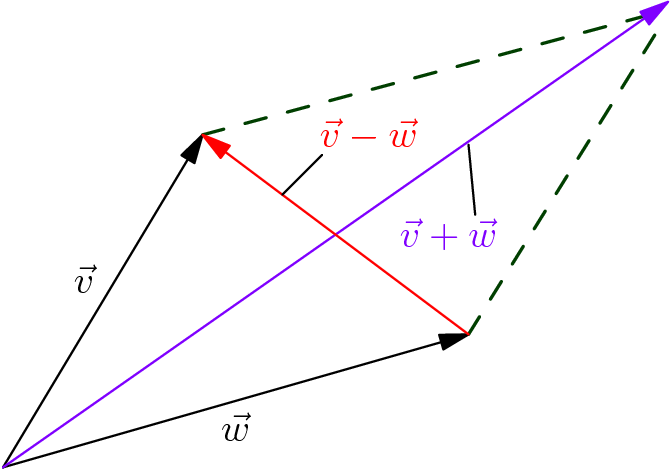
\includegraphics[scale=0.33]{Images/backgroundReview/Parallelogram}
\end{figure}

\noindent
We can also multiply vectors by scalars and get another vector as a result. We do this by multiplying each component of the vector by the scalar. This has the effect of stretching or shrinking the vector and possibly changing the vector's direction if the scalar is negative.

\begin{figure}[h]
	\centering
	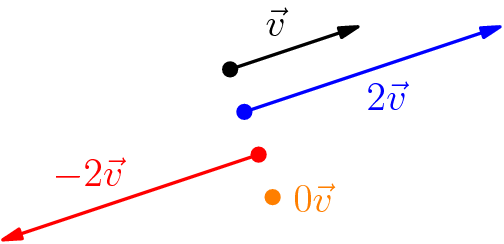
\includegraphics[scale=0.5]{Images/backgroundReview/ScalarMultiples}
\end{figure}

\noindent
A unit vector is any vector with magnitude 1. Rather than using an arrow like for other vectors, unit vectors are notated with a carat (\^) over top, like $\hat{i}$, which is read as "i hat".\\
We an transform any vector with non-zero magnitude into a unit vector by dividing the vector by its norm. This normalized vector will point in the same direction as the original vector.\\

\noindent
It is common in mathematics for $\hat{i}=\langle 1,0,0 \rangle$ to be the unit vector in the x-direction, $\hat{j}=\langle 0,1,0 \rangle$ to be the unit vector in the y-direction, and $\hat{k}=\langle 0,0,1 \rangle$ to be the unit vector in the z-direction.\\
Together, $\hat{i}$, $\hat{j}$, and $\hat{k}$ are called the standard basis vectors because all other vectors can be written as linear combination of these.

\begin{figure}[h]
	\centering
	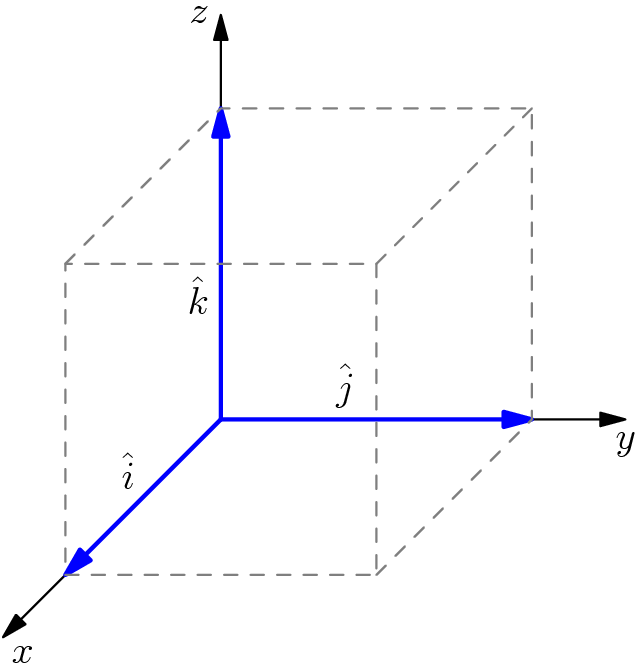
\includegraphics[scale=0.33]{Images/backgroundReview/UnitVectors}
\end{figure}

\subsection{Dot Products}
\noindent
A dot product is a way of multiplying two vectors so that the result is a scalar.
$\vec{a}\cdot\vec{b} = \norm{\vec{a}}\norm{\vec{b}}\cos{\theta}$ where $\theta$ is the angle between $\vec{a}$ and $\vec{b}$.
One way to think of the dot product is as a measure of how much two vectors point in the same direction.
We can also show using the law of cosines that $\vec{a}\cdot\vec{b} = a_1b_1+a_2b_2+...+a_nb_n$.
Knowing the lengths of two vectors and their dot product we can calculate the angle between them as
\begin{equation*}
	\theta = \arccos{\left(\frac{\vec{a} \cdot \vec{b}}{\norm{\vec{a}} \norm{\vec{b}}}\right)}.
\end{equation*}

\begin{figure}[H]
	\centering
	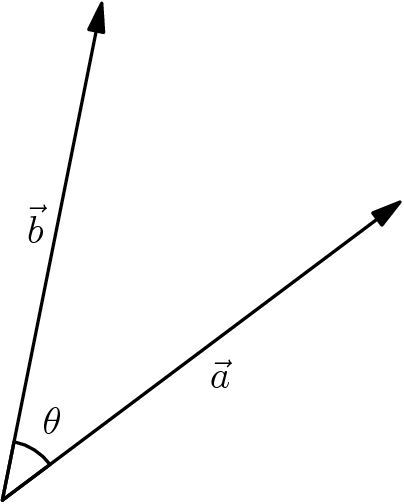
\includegraphics[width=0.25\textwidth]{./Images/backgroundReview/DotProduct.png}
	\caption{Two vectors and the angle between them}
\end{figure}

\noindent
Although similar to scalar multiplication, dot products have some properties that set them apart.
\begin{enumerate}[label=]
	\item \textbf{Commutative}
		\begin{equation*}
			\vec{a}\cdot\vec{b} = \vec{b}\cdot\vec{a}
		\end{equation*}
		the same as scalar multiplication.
	\item \textbf{Distributive}
		\begin{equation*}
			\vec{a}\cdot\left(\vec{b}+\vec{c}\right) = \vec{a}\cdot\vec{b}+\vec{a}\cdot\vec{c}
		\end{equation*}
		the same as scalar multiplication.
	\item \textbf{\underline{NOT} Associative}
		$\left(\vec{a}\cdot\vec{b}\right)\cdot\vec{c}$ is a nonsense expression.
		However, like scalar multiplication, dot products are scalar associative.
		\begin{equation*}
			\left(c\cdot\vec{a}\right)\cdot\vec{b} = \vec{a}\cdot\left(c\cdot\vec{b}\right)
		\end{equation*}
\end{enumerate}
\subsection{Cross Products}
\noindent
A cross product is a way of multiplying two vectors so that the result is a vector. Although the cross product technically only works for 3D vectors, we will first look a a "fake" 2D version to build an intuition.
\begin{equation*}
	\vec{a}\times\vec{b} = a_1b_1-a_2b_2
\end{equation*}
This "fake" 2D cross product gives the area of the parallelogram spanned by $\vec{a}$ and $\vec{b}$.
\begin{equation*}
	\vec{a}\times\vec{b} = \norm{\vec{a}}\norm{\vec{b}}\sin{\theta}	
\end{equation*}
where $\theta$ is the angle between $\vec{a}$ and $\vec{b}$.\\
Another way to think of the magnitude of the cross product, both in 2D and 3D, is as a measure of how perpendicular two vectors are.

\begin{figure}[H]
	\centering
	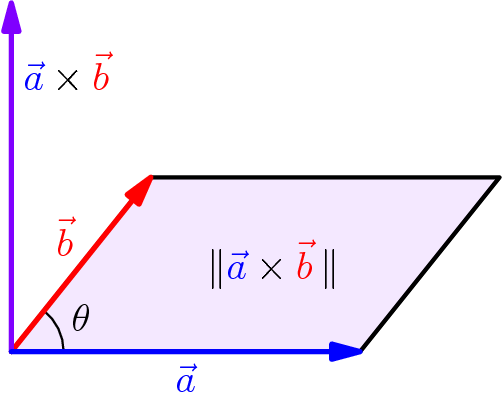
\includegraphics[scale=0.5]{Images/backgroundReview/CrossProduct}
\end{figure}

\noindent
In 3D, $\vec{a}\times\vec{b}$ is a vector, and similar to the 2D case, the magnitude of $\vec{a}\times\vec{b}$ is equal to the area of the parallelogram spanned by $\vec{a}$ and $\vec{b}$.
\begin{equation*}
	\vec{a}\times\vec{b} = \langle a_2b_3-b_2a_3,a_3b_1-b_3a_1,a_1b_2-b_1a_2 \rangle
\end{equation*}
and
\begin{equation*}
	\norm{\vec{a}\times\vec{b}}=\norm{\vec{a}}\norm{\vec{b}}\sin{\theta}
\end{equation*}
where $\theta$ is the angle between $\vec{a}$ and $\vec{b}$.\\
Each component of $\vec{a}\times\vec{b}$ gives the area of the parallelogram spanned by $\vec{a}$ and $\vec{b}$ in some plane: The x-component of $\vec{a}\times\vec{b}$ gives the area in the yz-plane (x = 0 plane).\\
$\vec{a}\times\vec{b}$ is perpendicular, also called "normal," to the plane containing $\vec{a}$ and $\vec{b}$. It's direction, is determined by the right hand rule.\\

\noindent
The cross product table of the standard basis vectors is useful for providing some insight into the properties of the cross product.
\begin{table}[h]
	\centering
	\renewcommand{\arraystretch}{1.5}
	\begin{tabular}{|l|l|l|l|}
		\hline
		$\overrightarrow{\text{row}}\times\overrightarrow{\text{col}}$ & $\hat{i}$  & $\hat{j}$  & $\hat{k}$  \\ \hline
		$\hat{i}$                                & $0$        & $\hat{k}$  & $-\hat{j}$ \\ \hline
		$\hat{j}$                                & $-\hat{k}$ & $0$        & $\hat{i}$  \\ \hline
		$\hat{k}$                                & $\hat{j}$  & $-\hat{i}$ & $0$        \\ \hline
	\end{tabular}
\end{table}

\begin{itemize}
	\item \textbf{NOT} Commutative, but is antisymmetric
	\begin{equation*}
		\vec{a}\times\vec{b} = -\left(\vec{b}\times\vec{a}\right)
	\end{equation*}
	\item Scalar Associative
	\begin{equation*}
		\left(c\cdot\vec{a}\right)\times\vec{b}=\vec{a}\times\left(c\cdot\vec{b}\right)
	\end{equation*}
	\item Distributive
	\begin{equation*}
		\vec{a}\times\left(\vec{b}\times\vec{c}\right) = \vec{a}\times\vec{b} + \vec{a}\times\vec{c}
	\end{equation*}
\end{itemize}

\noindent
One can also think of the cross product as the determinant of a matrix.
\begin{equation*}
	\vec{a}\times\vec{b} = \det\begin{bmatrix}
		\hat{i}& \hat{j} & \hat{k} \\
		a_1 & a_2 & a_2\\
		b_1 & b_2 & b_3 
	\end{bmatrix}
\end{equation*}

\noindent
Now that we have defined the dot product and cross product, we can put the two together as the scalar triple product, which gives the volume of the parallelepiped spanned by $\vec{a}$, $\vec{b}$, and $\vec{c}$.\\
\begin{center}
	$\vec{a}\cdot\left(\vec{b}\times\vec{c}\right)=\left|\begin{matrix}a_1 & a_2 & a_2\\b_1 & b_2 & b_3 \\ c_1 & c_2 & c_3\end{matrix}\right|$
\end{center}

\begin{figure}[h]
	\centering
	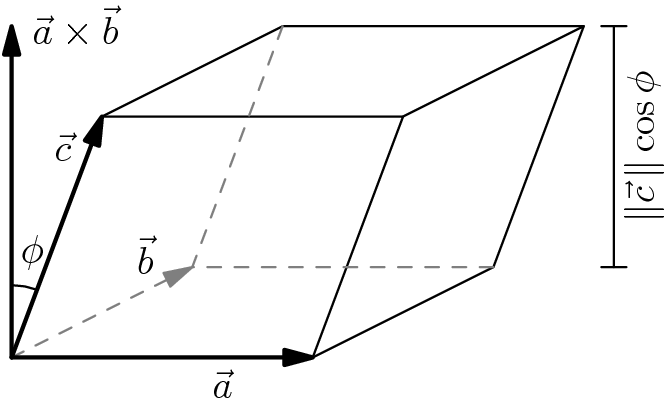
\includegraphics[scale=0.29]{Images/backgroundReview/Parallelipiped}
\end{figure}
